% !TeX root = ..\literaturereview.tex

\section{Gaussian processes}

One proposed way to better understand \ac{DL} is by using \acp{GP} to approximate the output of a \ac{DL} algorithm.

In a similar way to how a univariate normal distribution with a mean and variance can be generalised to a multivariate normal distribution with a mean vector and a normal vector, a \ac{GP} is the limit of extending a multivariate normal distribution to infinite dimensions, with a mean function and covariance function (sometimes also called a kernel in ML environments) which depends on the distance between two points.

A random vector \(X \in \reals{}^n\) is distributed with a multivariate normal distribution in \(n\) dimensions with mean vector \(\vec{\mu} \in \reals{}^n\) and covariance matrix \(K \in \reals^{n \times n}\) if \(X \distributed \normdist(\vec{\mu},\, K)\).
In a similar way, \(Y\) is a \ac{GP} with a mean function \(\mu(\x)\) and a covariance function \(k(\x{}, \x{})\) where \(k(x_1, x_2) = k(\left|x_1-x_2\right|)\) if \(Y \distributed \gp(\mu,\, k)\).
Because a \ac{GP} is an extension of a multivariate normal distribution, any finite subset of points from a \ac{GP} has a multivariate normal distribution~\autocite[515]{williams1996}.

\subsection{History of Gaussian processes}

\acp{GP} have been independently rediscovered many times in the 20th century in the contexts of time series, physics, mining, meteorology, computer experiments and machine learning~\autocite[2]{mackay1997}.

\subsubsection{Time series}

The origins of \acp{GP} can be traced at least as far back as WWII, and the work of \textcite{wold1938} and \textcite{wiener1949} on time series.
They developed ARMA models and spline smoothing, which correspond to one dimensional \acp{GP} with specific choices of covariance functions.

\subsubsection{Krige}

In the 1950s, the problem of mine valuation --- the decision of where to establish a gold mine --- was often based on the sample mean and sample standard deviation of repeated biased sampling of the ore grade in an area.
However, this simple statistical method could not accurately predict the volume of ore in an area and did not capture the variability of the ore density~\autocites[244]{cressie1990}[119]{krige1951}.
Many datapoints were needed to reduce the estimate of the ore density's variance to an acceptable level, and so often an insufficient number of samples were taken or money was wasted on taking too many samples.
South African mining engineer and geostatistician Danie Krige\footnote{Afrikaans pronunciation: \textipa{[dAni: "kriX@]}} proposed some improvements to these methods, one of which was to take into account the distance of the samples from each other, which greatly reduced the number of samples needed~\autocite{krige1951}.

Despite the advantages of his ideas over the simpler techniques, his methods were still flawed.
When estimating a value at a specific location \(\vec{x}\), Krige's method weighted the datapoints by their distance from \(\vec{x}\).
However, he weighted all points at a distance greater than some threshold with zero weight and all other points with an equal weight, rather than weighting the datapoints proportionally to their distance from the point being estimated~\autocite[245]{cressie1990}.
Krige later also experimented with including more points in his calculations, but did not put a smaller weight on more distant points, and so concluded that \qtc[362]{krige1962}{the advantage gained is of no practical significance}.
Krige also used ordinary least squares regression where generalised least squares regression is the optimum for correlated squared errors, although for the large datasets Krige worked with, the inaccuracy caused was minimal.

\subsubsection{Matheron}

Krige did not see the value in weighting individual datapoints, saying \qtc[125]{krige1951}{any sample value cannot be regarded as having a so-called \qt{area or distance of influence,} in the generally accepted sense}.
In the 1960s, French mathematician and geostatistician Georges Matheron formalised Krige's work and greatly expanded on it, coining the term \qt{krigeage} (later anglicised to \qt{kriging})~\autocite{matheron1960} and founding the field of geostatistics.

Matheron's way of formalising the \qt{area of influence} that Krige had dismissed was to create a function called the \qt{variogram}, which represents the dissimilarity between two points and should increase as the distance between the points increases.
\qtc[1250]{matheron1963}{[The variogram] gives a precise content to the traditional concept of the influence zone of a sample}.
He defined the variogram \(2\gamma(\x, \x)\) as the variance of the difference between two points:
\[ 2\gamma(\vec{x}_i, \vec{x}_j) = \operatorname{Var}\left(y(\vec{x}_i) - y(\vec{x}_j)\right). \]

The semivariogram \(\gamma(\x,\x)\) is half of the variogram and helps define how similarity behaves as distance between points changes.
The \qt{nugget effect} is so named to reflect the fact that if gold has been found at a specific location, the probability of finding gold within a very small distance is also 1, i.e.\ still inside the gold nugget.
For data points, the nugget represents a measure of the variability between points at zero distance from each other.
Any variation at a distance less than the smallest sampling distance will be included in the nugget.
The \qt{range} represents the maximum distance at which similarity stops decreasing, and the \qt{sill} represents the level of dissimilarity between points at a distance greater than the range.

Fitting a curve to a semivariogram plot such as Figure~\ref{variogram} can be used to model the covariance function~\autocite[305]{diggle2002} as the covariance function \(k(\x, \x)\) is related to the semivariogram \(\gamma(\x, \x)\) by:
\[ \gamma(\vec{x}_i, \vec{x}_j) = \text{sill} - k(\vec{x}_i, \vec{x}_j). \]

\begin{figure}[htbp]
\centering
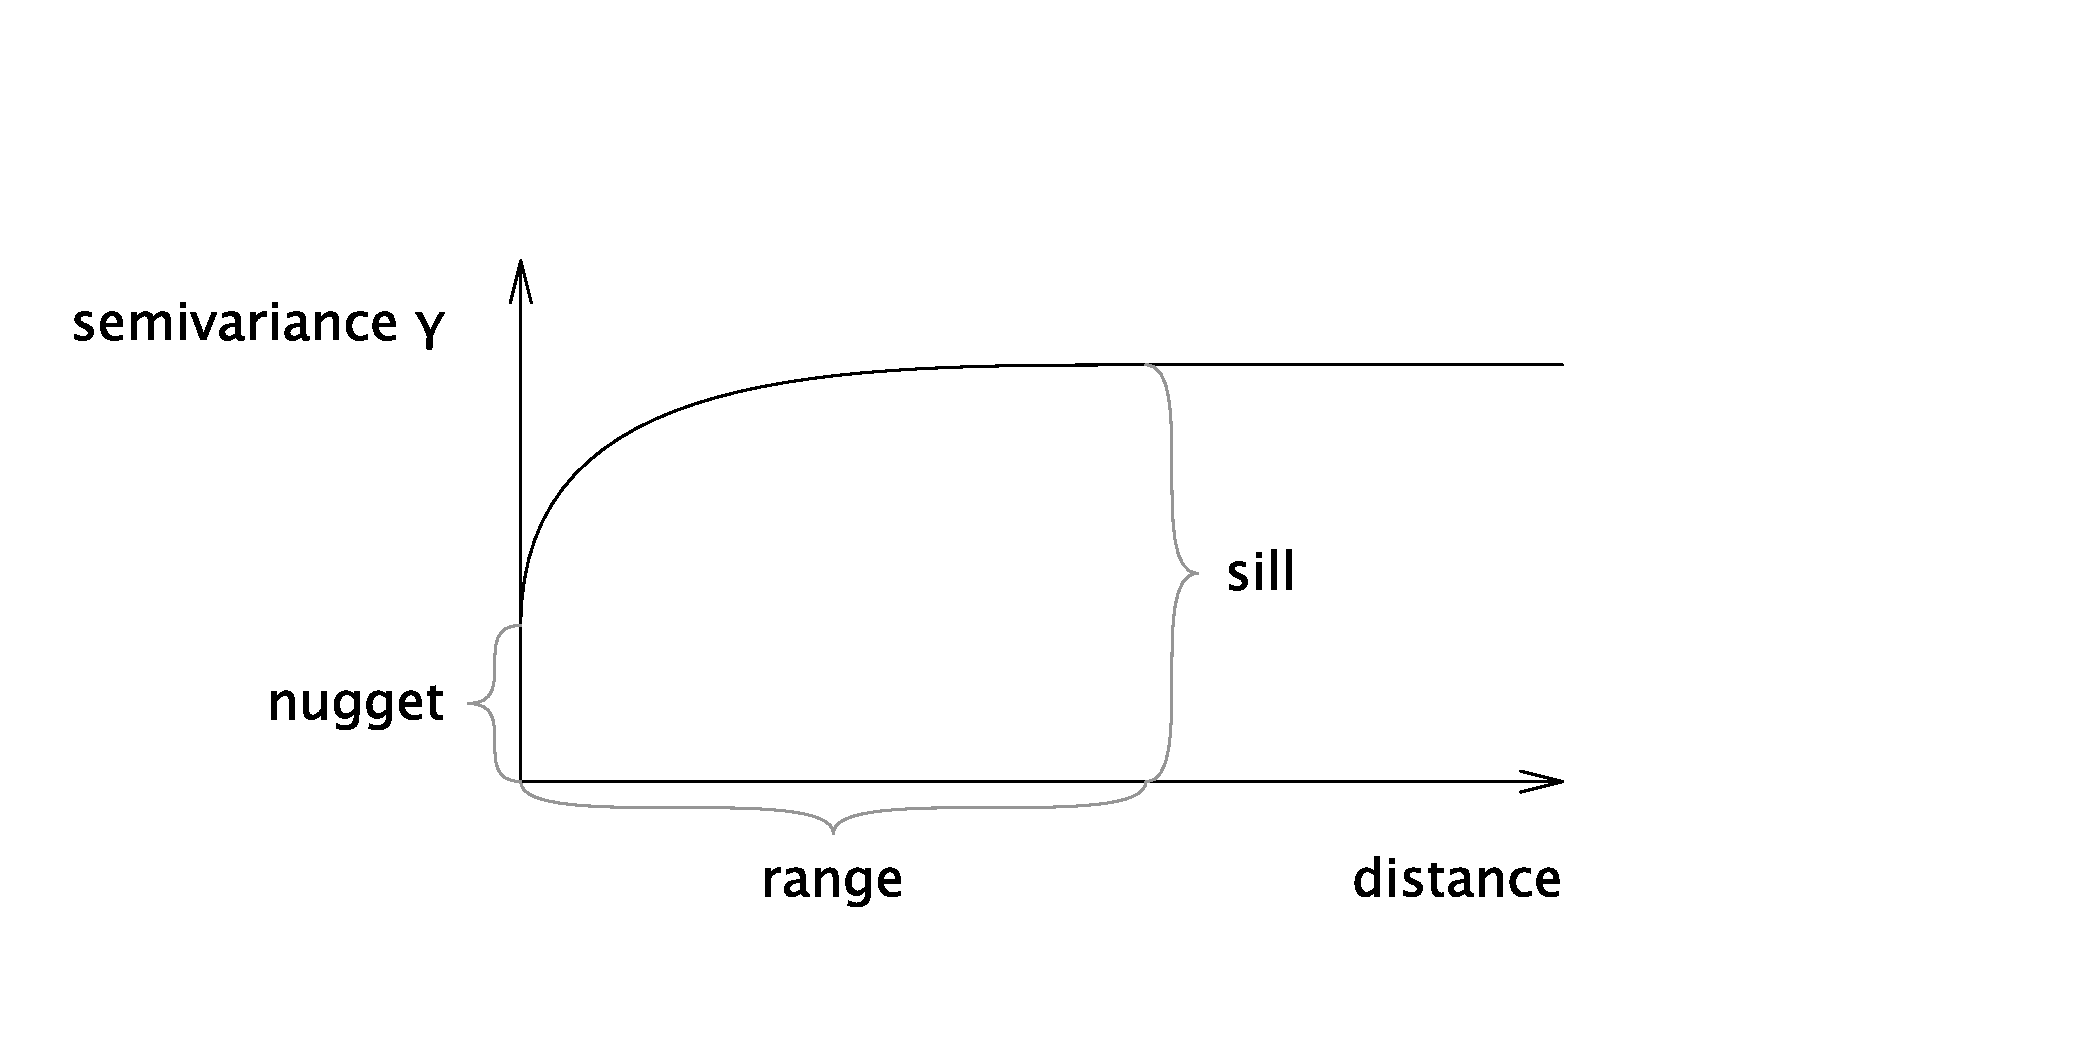
\includegraphics[width=\textwidth]{variogram.pdf}
\caption{An example theoretical semivariogram plot showing the nugget, range and sill.}
\label{variogram}
\end{figure}

As well as Krige, Matheron also was influenced by \textcite[translated into English in 1966]{gandin1963}.
This work was from the perspective of meteorology, Gandin's focus was more on the covariance function, whereas Matheron's geostatistics perspective meant he focused more on the variogram and semivariogram.

In \citeyear{philip1986}, \citeauthor{philip1986} criticised Matheron's work and the field of Matheronian geostatistics from the perspective of geologists.
They claimed the assumption of stationarity for ore density data was unrealistic~\autocite[86--87]{philip1986} and that least squares regression was inappropriate because of its assumption of normality~\autocite[101--102]{philip1986} and the disproportionate effect of outliers on the estimates~\autocite[102]{philip1986}.

\subsection{Computer experiments}

Another field in which \acp{GP} have been heavily used is in computer experiments, where the techniques were generalised to both more contexts and higher dimensions than two and three dimensional geostatistics.
Instead of expensive physical experiments, large models are used to model physical phenomena such as circuit design, nuclear fusion, plant ecology, and thermal energy storage~\autocite[409]{sacks1989}, usually involving large sets of differential equations.
In cases such as weather, physical experimentation is impossible, so the only option is to solve these models by a complex computer program, which can be very computationally expensive, taking hours or days to complete a single run.
It is therefore infeasible to complete multiple runs of the model with the same inputs for use in Monte Carlo simulations to calculate uncertainty like one would with a physical experiment.
Additionally, the models are often deterministic, so even if multiple runs can be performed, the uncertainty in the estimate cannot be measured.
One method to overcome these limitations is to run the computer model with a variety of input parameters and treat the outcomes as realisations of a \ac{GP} model~\autocite[163]{bachoc2017}
This allows for interpolation of the model's outputs and quantification of the associated uncertainty of the computer model.

\subsection{Modern trends}

Modern trends in the field of \acp{GP} include \acp{GP} for big data, where the number of datapoints can be many millions or billions~\autocite{hensman2013}.
This means that traditional methods which involve inverting an \(n \times n\) matrix cannot be used.

Deep \acp{GP} (or hierarchical \acp{GP}) are analogous to deep neural networks (see Section~\ref{deeplearning}), and involve chaining the output of one \ac{GP} into another to stronger model nonlinearity in the data~\autocite{damianou2013}.
